\PassOptionsToPackage{unicode=true}{hyperref} % options for packages loaded elsewhere
\PassOptionsToPackage{hyphens}{url}
%
\documentclass[]{book}
\usepackage{lmodern}
\usepackage{amssymb,amsmath}
\usepackage{ifxetex,ifluatex}
\usepackage{fixltx2e} % provides \textsubscript
\ifnum 0\ifxetex 1\fi\ifluatex 1\fi=0 % if pdftex
  \usepackage[T1]{fontenc}
  \usepackage[utf8]{inputenc}
  \usepackage{textcomp} % provides euro and other symbols
\else % if luatex or xelatex
  \usepackage{unicode-math}
  \defaultfontfeatures{Ligatures=TeX,Scale=MatchLowercase}
\fi
% use upquote if available, for straight quotes in verbatim environments
\IfFileExists{upquote.sty}{\usepackage{upquote}}{}
% use microtype if available
\IfFileExists{microtype.sty}{%
\usepackage[]{microtype}
\UseMicrotypeSet[protrusion]{basicmath} % disable protrusion for tt fonts
}{}
\IfFileExists{parskip.sty}{%
\usepackage{parskip}
}{% else
\setlength{\parindent}{0pt}
\setlength{\parskip}{6pt plus 2pt minus 1pt}
}
\usepackage{hyperref}
\hypersetup{
            pdftitle={Making Lecture Notes with Bookdown},
            pdfauthor={Vicky Scowcroft},
            pdfborder={0 0 0},
            breaklinks=true}
\urlstyle{same}  % don't use monospace font for urls
\usepackage{color}
\usepackage{fancyvrb}
\newcommand{\VerbBar}{|}
\newcommand{\VERB}{\Verb[commandchars=\\\{\}]}
\DefineVerbatimEnvironment{Highlighting}{Verbatim}{commandchars=\\\{\}}
% Add ',fontsize=\small' for more characters per line
\usepackage{framed}
\definecolor{shadecolor}{RGB}{248,248,248}
\newenvironment{Shaded}{\begin{snugshade}}{\end{snugshade}}
\newcommand{\AlertTok}[1]{\textcolor[rgb]{0.94,0.16,0.16}{#1}}
\newcommand{\AnnotationTok}[1]{\textcolor[rgb]{0.56,0.35,0.01}{\textbf{\textit{#1}}}}
\newcommand{\AttributeTok}[1]{\textcolor[rgb]{0.77,0.63,0.00}{#1}}
\newcommand{\BaseNTok}[1]{\textcolor[rgb]{0.00,0.00,0.81}{#1}}
\newcommand{\BuiltInTok}[1]{#1}
\newcommand{\CharTok}[1]{\textcolor[rgb]{0.31,0.60,0.02}{#1}}
\newcommand{\CommentTok}[1]{\textcolor[rgb]{0.56,0.35,0.01}{\textit{#1}}}
\newcommand{\CommentVarTok}[1]{\textcolor[rgb]{0.56,0.35,0.01}{\textbf{\textit{#1}}}}
\newcommand{\ConstantTok}[1]{\textcolor[rgb]{0.00,0.00,0.00}{#1}}
\newcommand{\ControlFlowTok}[1]{\textcolor[rgb]{0.13,0.29,0.53}{\textbf{#1}}}
\newcommand{\DataTypeTok}[1]{\textcolor[rgb]{0.13,0.29,0.53}{#1}}
\newcommand{\DecValTok}[1]{\textcolor[rgb]{0.00,0.00,0.81}{#1}}
\newcommand{\DocumentationTok}[1]{\textcolor[rgb]{0.56,0.35,0.01}{\textbf{\textit{#1}}}}
\newcommand{\ErrorTok}[1]{\textcolor[rgb]{0.64,0.00,0.00}{\textbf{#1}}}
\newcommand{\ExtensionTok}[1]{#1}
\newcommand{\FloatTok}[1]{\textcolor[rgb]{0.00,0.00,0.81}{#1}}
\newcommand{\FunctionTok}[1]{\textcolor[rgb]{0.00,0.00,0.00}{#1}}
\newcommand{\ImportTok}[1]{#1}
\newcommand{\InformationTok}[1]{\textcolor[rgb]{0.56,0.35,0.01}{\textbf{\textit{#1}}}}
\newcommand{\KeywordTok}[1]{\textcolor[rgb]{0.13,0.29,0.53}{\textbf{#1}}}
\newcommand{\NormalTok}[1]{#1}
\newcommand{\OperatorTok}[1]{\textcolor[rgb]{0.81,0.36,0.00}{\textbf{#1}}}
\newcommand{\OtherTok}[1]{\textcolor[rgb]{0.56,0.35,0.01}{#1}}
\newcommand{\PreprocessorTok}[1]{\textcolor[rgb]{0.56,0.35,0.01}{\textit{#1}}}
\newcommand{\RegionMarkerTok}[1]{#1}
\newcommand{\SpecialCharTok}[1]{\textcolor[rgb]{0.00,0.00,0.00}{#1}}
\newcommand{\SpecialStringTok}[1]{\textcolor[rgb]{0.31,0.60,0.02}{#1}}
\newcommand{\StringTok}[1]{\textcolor[rgb]{0.31,0.60,0.02}{#1}}
\newcommand{\VariableTok}[1]{\textcolor[rgb]{0.00,0.00,0.00}{#1}}
\newcommand{\VerbatimStringTok}[1]{\textcolor[rgb]{0.31,0.60,0.02}{#1}}
\newcommand{\WarningTok}[1]{\textcolor[rgb]{0.56,0.35,0.01}{\textbf{\textit{#1}}}}
\usepackage{longtable,booktabs}
% Fix footnotes in tables (requires footnote package)
\IfFileExists{footnote.sty}{\usepackage{footnote}\makesavenoteenv{longtable}}{}
\usepackage{graphicx,grffile}
\makeatletter
\def\maxwidth{\ifdim\Gin@nat@width>\linewidth\linewidth\else\Gin@nat@width\fi}
\def\maxheight{\ifdim\Gin@nat@height>\textheight\textheight\else\Gin@nat@height\fi}
\makeatother
% Scale images if necessary, so that they will not overflow the page
% margins by default, and it is still possible to overwrite the defaults
% using explicit options in \includegraphics[width, height, ...]{}
\setkeys{Gin}{width=\maxwidth,height=\maxheight,keepaspectratio}
\setlength{\emergencystretch}{3em}  % prevent overfull lines
\providecommand{\tightlist}{%
  \setlength{\itemsep}{0pt}\setlength{\parskip}{0pt}}
\setcounter{secnumdepth}{5}
% Redefines (sub)paragraphs to behave more like sections
\ifx\paragraph\undefined\else
\let\oldparagraph\paragraph
\renewcommand{\paragraph}[1]{\oldparagraph{#1}\mbox{}}
\fi
\ifx\subparagraph\undefined\else
\let\oldsubparagraph\subparagraph
\renewcommand{\subparagraph}[1]{\oldsubparagraph{#1}\mbox{}}
\fi

% set default figure placement to htbp
\makeatletter
\def\fps@figure{htbp}
\makeatother

\usepackage{booktabs}
\usepackage{amsthm}
\makeatletter
\def\thm@space@setup{%
  \thm@preskip=8pt plus 2pt minus 4pt
  \thm@postskip=\thm@preskip
}
\makeatother
\usepackage[]{natbib}
\bibliographystyle{plainnat}

\title{Making Lecture Notes with Bookdown}
\author{Vicky Scowcroft}
\date{2020-08-27}

\begin{document}
\maketitle

{
\setcounter{tocdepth}{1}
\tableofcontents
}
\hypertarget{introduction}{%
\chapter*{Introduction}\label{introduction}}
\addcontentsline{toc}{chapter}{Introduction}

This guide walks through how to create html lecture notes using \textbf{R}, \textbf{Markdown} and \textbf{Bookdown}. This format is preferred as LaTeX doesn't play nicely with accessibility tools like screen readers, especially for maths heavy content.

\hypertarget{system-requirements}{%
\section*{System Requirements}\label{system-requirements}}
\addcontentsline{toc}{section}{System Requirements}

To use bookdown, you will need to have R and R studio installed (perhaps R studio is not a requirement, but it makes things a lot easier). These can both be installed from the DDAT Self Service app on a Mac, or R can be downloaded directly from \href{https://cran.r-project.org/}{here} and R Studio from \href{https://rstudio.com/products/rstudio/download/}{here}. You will also need \href{https://pandoc.org/index.html}{\textbf{pandoc}}. This may already be installed on your system as part of the Anaconda distribution.

The \href{https://bookdown.org/yihui/bookdown/}{\textbf{bookdown}} package can be installed from CRAN or Github:

\begin{Shaded}
\begin{Highlighting}[]
\KeywordTok{install.packages}\NormalTok{(}\StringTok{"bookdown"}\NormalTok{)}
\CommentTok{# or the development version}
\CommentTok{# devtools::install_github("rstudio/bookdown")}
\end{Highlighting}
\end{Shaded}

\hypertarget{caveat}{%
\section*{Caveat}\label{caveat}}
\addcontentsline{toc}{section}{Caveat}

The instructions in this guide are what worked for me, on a Mac using R version 4.0.2, R Studio version 1.3 and pandoc version 2.2.3.2. This guide also assumes that you're familiar with using the command line.

\hypertarget{getting-started}{%
\chapter{Getting started}\label{getting-started}}

The quickest way to get started is to use the bookdown demo as a template. \href{https://bookdown.org/yihui/bookdown/get-started.html}{This page} gives instructions for how to do this.

The \href{https://bookdown.org/yihui/bookdown/}{bookdown: Authoring Books and Technical Documents with R Markdown} is the main documentation for bookdown. I won't repeat a lot of the information here.

This guide will walk through the steps I used to convert my LaTeX lecture notes for PH40112 to the bookdown version \href{https://vickyscowcroft.github.io/PH40112_rmd/}{here}. The files used to create the PH40112 notes are available on \href{https://github.com/vickyscowcroft/PH40112_rmd}{github} and you're welcome to use those as a starting point.

\hypertarget{convert-latex}{%
\chapter{Converting from LaTeX notes}\label{convert-latex}}

\hypertarget{sec:con-tex}{%
\section{Converting tex files}\label{sec:con-tex}}

If you already have LaTeX versions of your notes you can convert these to markdown using pandoc Pandoc won't create \emph{perfect} versions of your notes - you'll most likely have to do a bit of tweaking, but it gets most of the way there.

You can convert a tex file to Rmd via the command

\begin{verbatim}
pandoc -f latex -t markdown input-tex.tex -o output-md.Rmd
\end{verbatim}

where \texttt{input-tex.tex} is the name of your tex file and \texttt{output-md.Rmd} is the name of your output Rmd file.

Pandoc converts one tex file at a time. It doesn't understand how to process a ``master'' tex file with \texttt{input} or \texttt{insert} LaTeX commands. Each file will need to be processed separately.

\hypertarget{batch-conversion}{%
\section{Batch conversion}\label{batch-conversion}}

If you want to convert a batch of latex files you can script the process.

\hypertarget{tidying}{%
\section{Tidying up the Rmd file}\label{tidying}}

Pandoc will have done most of the work in getting your tex file converted to markdown. However, depending on how complex the original file was, you may end up with some tidying to do.

Things that typically will need fixing are:

\begin{itemize}
\tightlist
\item
  Section etc labels - if you used underscores in any of your latex labels you should change these to `-' in the markdown file. The underscores confuse markdown. Section \ref{sec:chapters} discusses sections, chapters, etc.
\item
  Figures - the default pandoc conversion is quite limited, so here we'll use a more adaptable figure environment. In practice its easiest to just copy-paste the example code in Chapter \ref{sec:figures} and edit the relavent bits.
\item
  Equations - the equations themselves should be fine, but if you want to have equation numbers you'll need to do some tidying. See Chapter \ref{sec:equations} for the syntax.
\item
  Tables - tables have a different format but it's pretty easy to convert a latex table using find/replace. See Chapter \ref{sec:tables}.
\item
  References - generally easy to fix. See Chapter \ref{sec:referencing}.
\end{itemize}

\hypertarget{sec:gaps}{%
\section{Notes with gaps}\label{sec:gaps}}

\textbf{Think carefully about whether you want to provide notes with gaps.} While they may serve a purpose when the students have a hard-copy of the notes in a live lecture, they will most likely be using your notes on a screen this year.

It is possible to create notes with gaps for things like equations etc for the students to fill in. To do this you need to add some extra code to the \texttt{index.Rmd} file:

\begin{verbatim}
```
{r setup, include=FALSE}
library(knitr)
knit_engines$set(asis = function(options) {
  if (options$echo && options$eval) knit_child(text = options$code)
})
```
\end{verbatim}

Then to ``hide'' e.g.~an equation but still keep the same numbering, edit your equation to the following format:

\begin{verbatim}
\begin{equation}
```{asis, echo=FALSE}
\Delta s^2 = \Delta x_{1}^{2} + \Delta x_{2}^{2}
```
\label{eq:dist01}
\end{equation}
\end{verbatim}

Here the \texttt{asis} command and back-ticks wrap around \textbf{only} the equation itself, rather than the whole \texttt{equation} object. If you wrap the \texttt{asis} around the \texttt{\textbackslash{}begin\{equation\}} and \texttt{\textbackslash{}end\{equation\}} the equation numbering will disappear too.

\hypertarget{sec:chapters}{%
\chapter{Chapters, sections, etc}\label{sec:chapters}}

\hypertarget{sec:file-structure}{%
\section{File Structure}\label{sec:file-structure}}

Bookdown organises your notes into a book. The main page you see when you open a bookdown page is the \texttt{index.Rmd} file.

Each chapter in the book has it's own markdown file. Each chapter filename should start with a number, and will be ordered numerically. For this book, the files are

\begin{Shaded}
\begin{Highlighting}[]
\NormalTok{index.Rmd}
\NormalTok{01-intro.Rmd}
\NormalTok{02-latex-conversion.Rmd}
\NormalTok{03-chapters.Rmd}
\NormalTok{... etc}
\end{Highlighting}
\end{Shaded}

\hypertarget{sec:headings}{%
\section{Headings}\label{sec:headings}}

The chapter title and label are given in the first line of the file.

\begin{Shaded}
\begin{Highlighting}[]
\FunctionTok{# Chapters, sections, etc \{#sec:chapters\}}
\end{Highlighting}
\end{Shaded}

The \texttt{\#} at the start of the line denotes a chapter heading. The label is given in \texttt{\{\#sec:chapters\}}.

You can make sections either using two \# at the start of the line, or with dashes under the section title:

\begin{Shaded}
\begin{Highlighting}[]
\NormalTok{Headings \{#sec:headings\}}
\NormalTok{--------}
\end{Highlighting}
\end{Shaded}

Note that the \texttt{\{\#sec:label\}} syntax is still the same - you don't need to say whether it's a chapter, section, subsection etc.

Subsections are done similarly, with either three \# at the start of the line.

You can change the section heading from `Chapter' to e.g.~section by editing the following in the \texttt{\_bookdown.yml} file:

\begin{Shaded}
\begin{Highlighting}[]
\NormalTok{language:}
\NormalTok{  ui:}
\BaseNTok{    chapter_name: "Section "}
\end{Highlighting}
\end{Shaded}

\hypertarget{sec:cross-ref}{%
\section{Cross referencing}\label{sec:cross-ref}}

You can reference other chapters, sections etc throughout the book with the following syntax:

\begin{Shaded}
\begin{Highlighting}[]
\NormalTok{Section \textbackslash{}@ref(sec:cross-ref) is this section.}
\end{Highlighting}
\end{Shaded}

Which shows up as ``Section \ref{sec:cross-ref} is this section.''.

When cross-referencing, you don't need the \# before \texttt{sec}. That's only used to define the label.

\hypertarget{sec:figures}{%
\chapter{Figures}\label{sec:figures}}

\hypertarget{sec:add-figs}{%
\section{Adding figures}\label{sec:add-figs}}

Figures and captions can be included, but the syntax is quite different to LaTeX.

Assuming that you would add a figure to a LaTeX document with the following code:

\begin{verbatim}
\begin{figure}
\begin{centering}
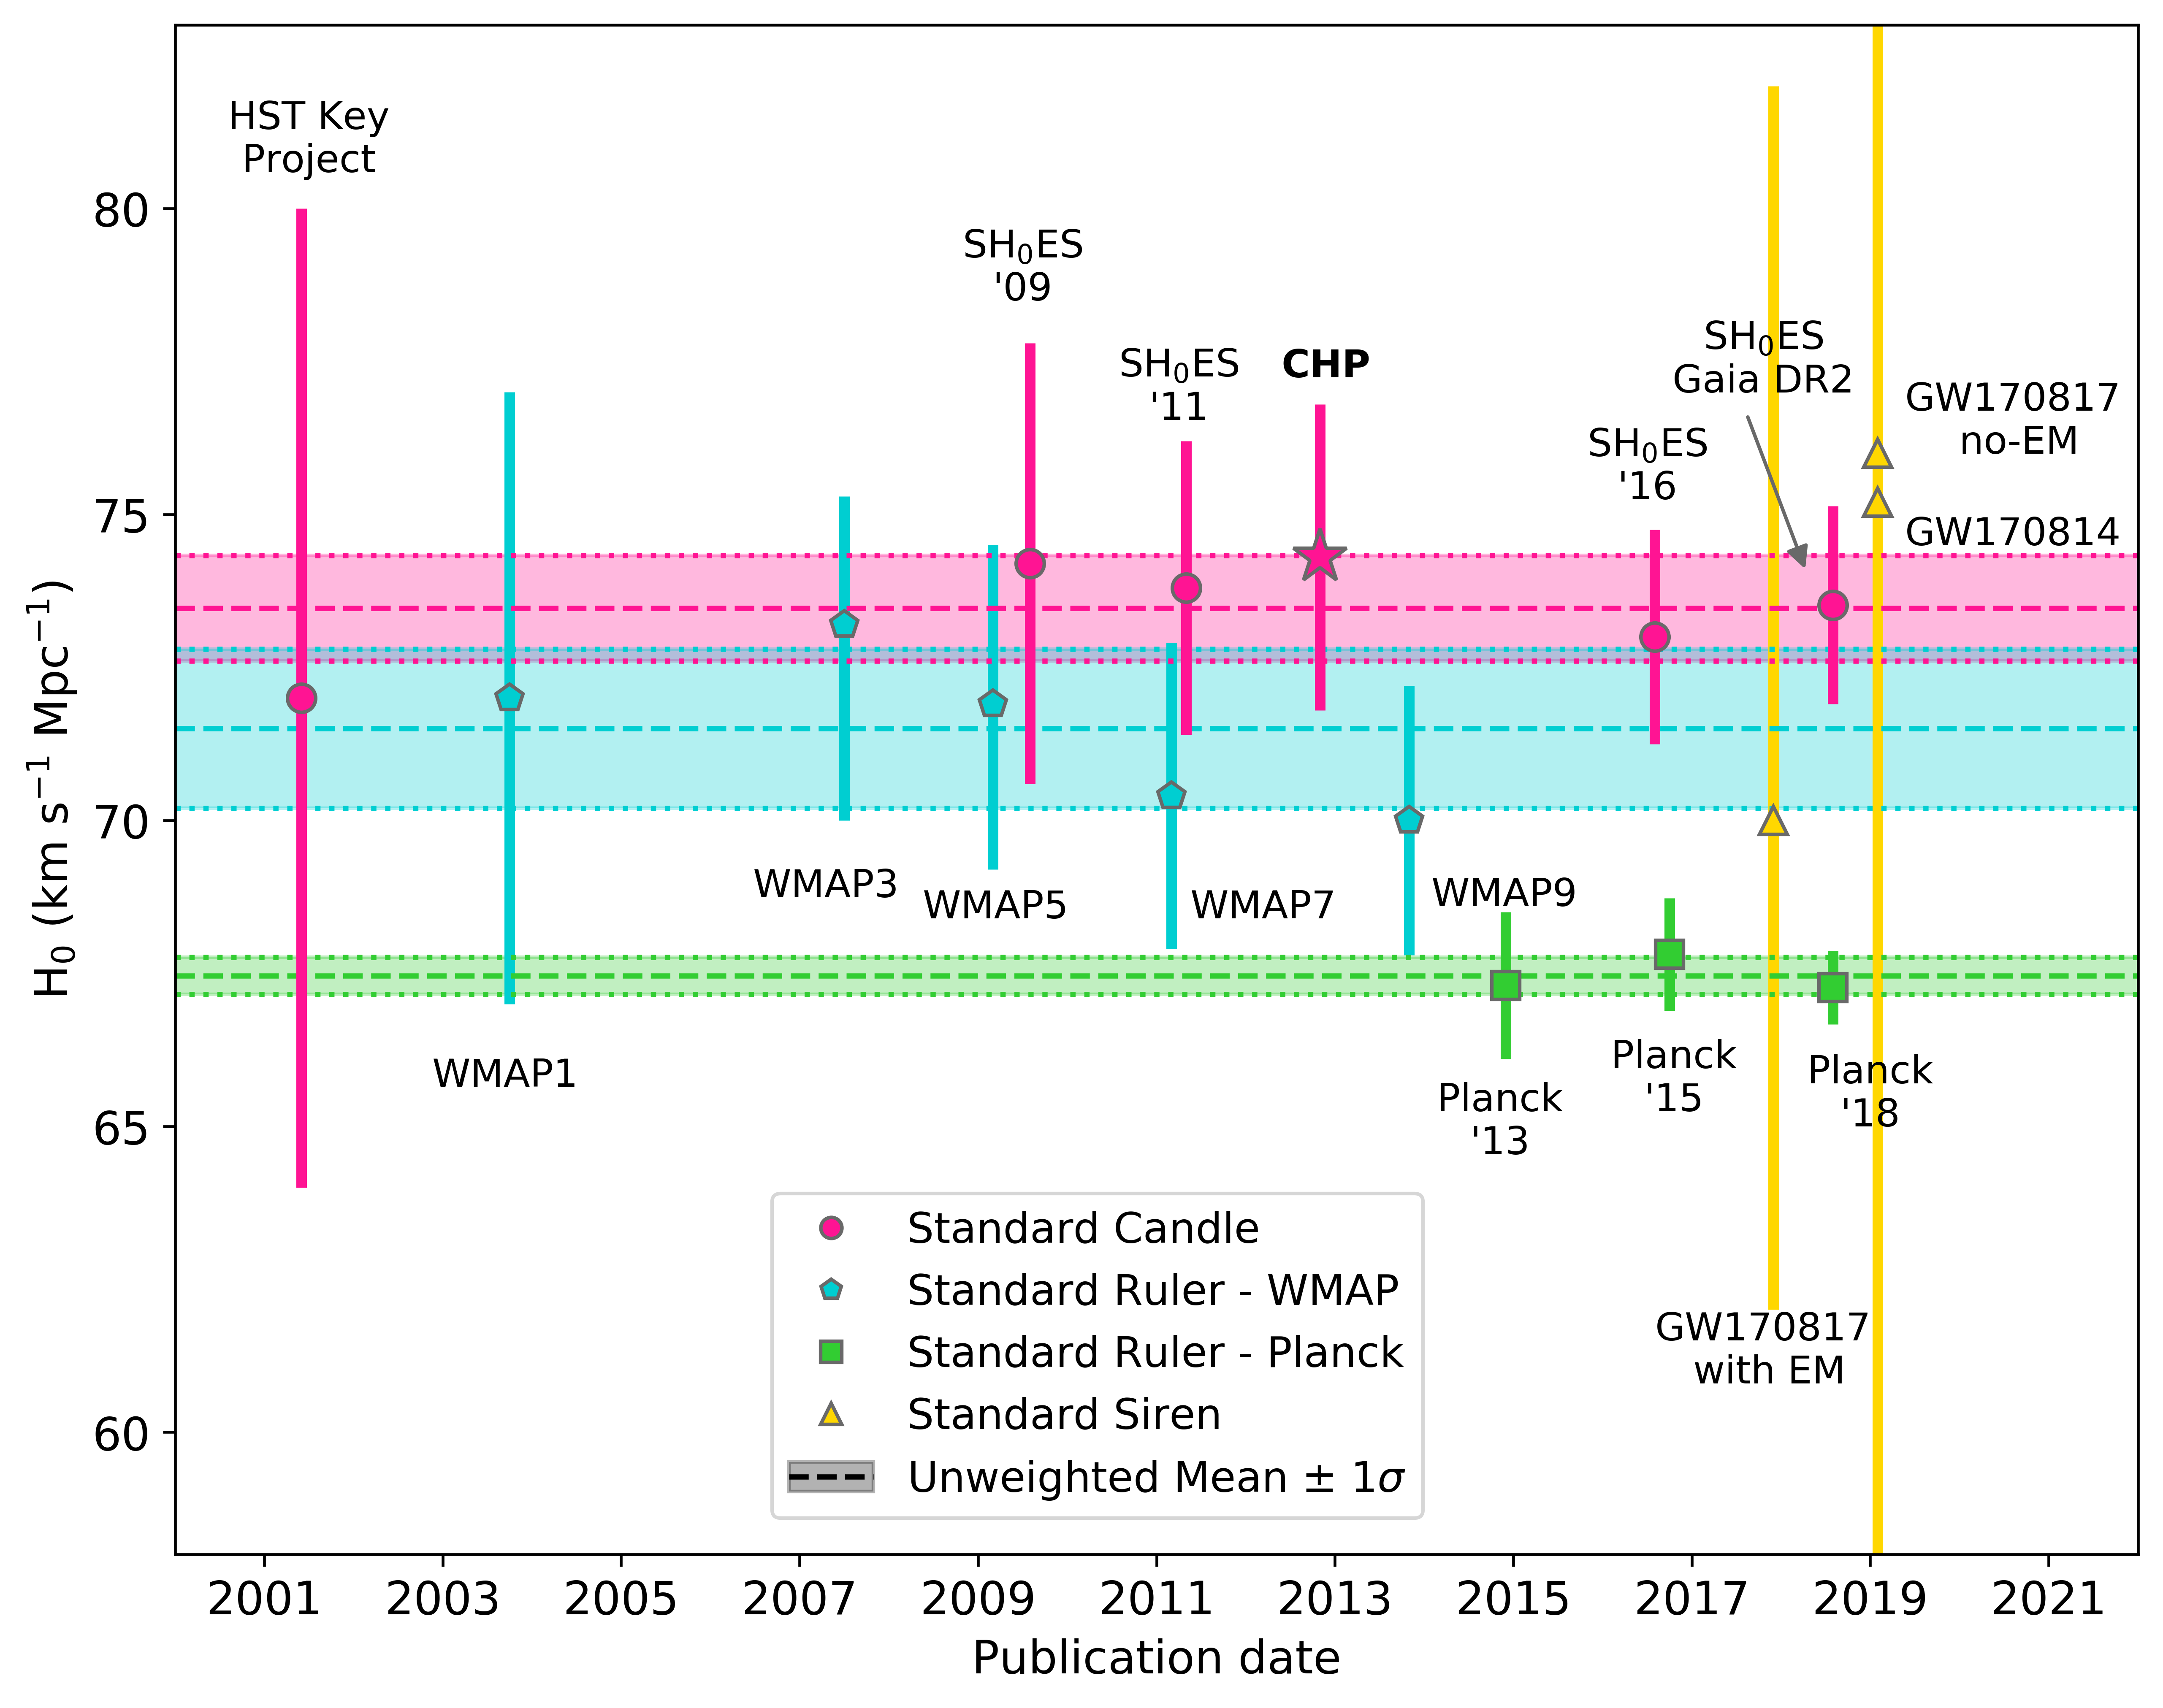
\includegraphics[width=0.7\textwidth]{Images/ho-tension.png}
\caption{This is a figure caption.}
\label{fig:ho-plot}
\end{centering}
\end{figure}
\end{verbatim}

To include the figure in markdown the syntax is as follows:

\begin{Shaded}
\begin{Highlighting}[]
\BaseNTok{```}
\BaseNTok{\{r echo=FALSE, ho-plot, out.width='70%', fig.show='hold', fig.cap="This is a figure caption."\}}
\BaseNTok{knitr::include_graphics("Images/ho-tension.png")}
\BaseNTok{```}
\end{Highlighting}
\end{Shaded}

\begin{figure}
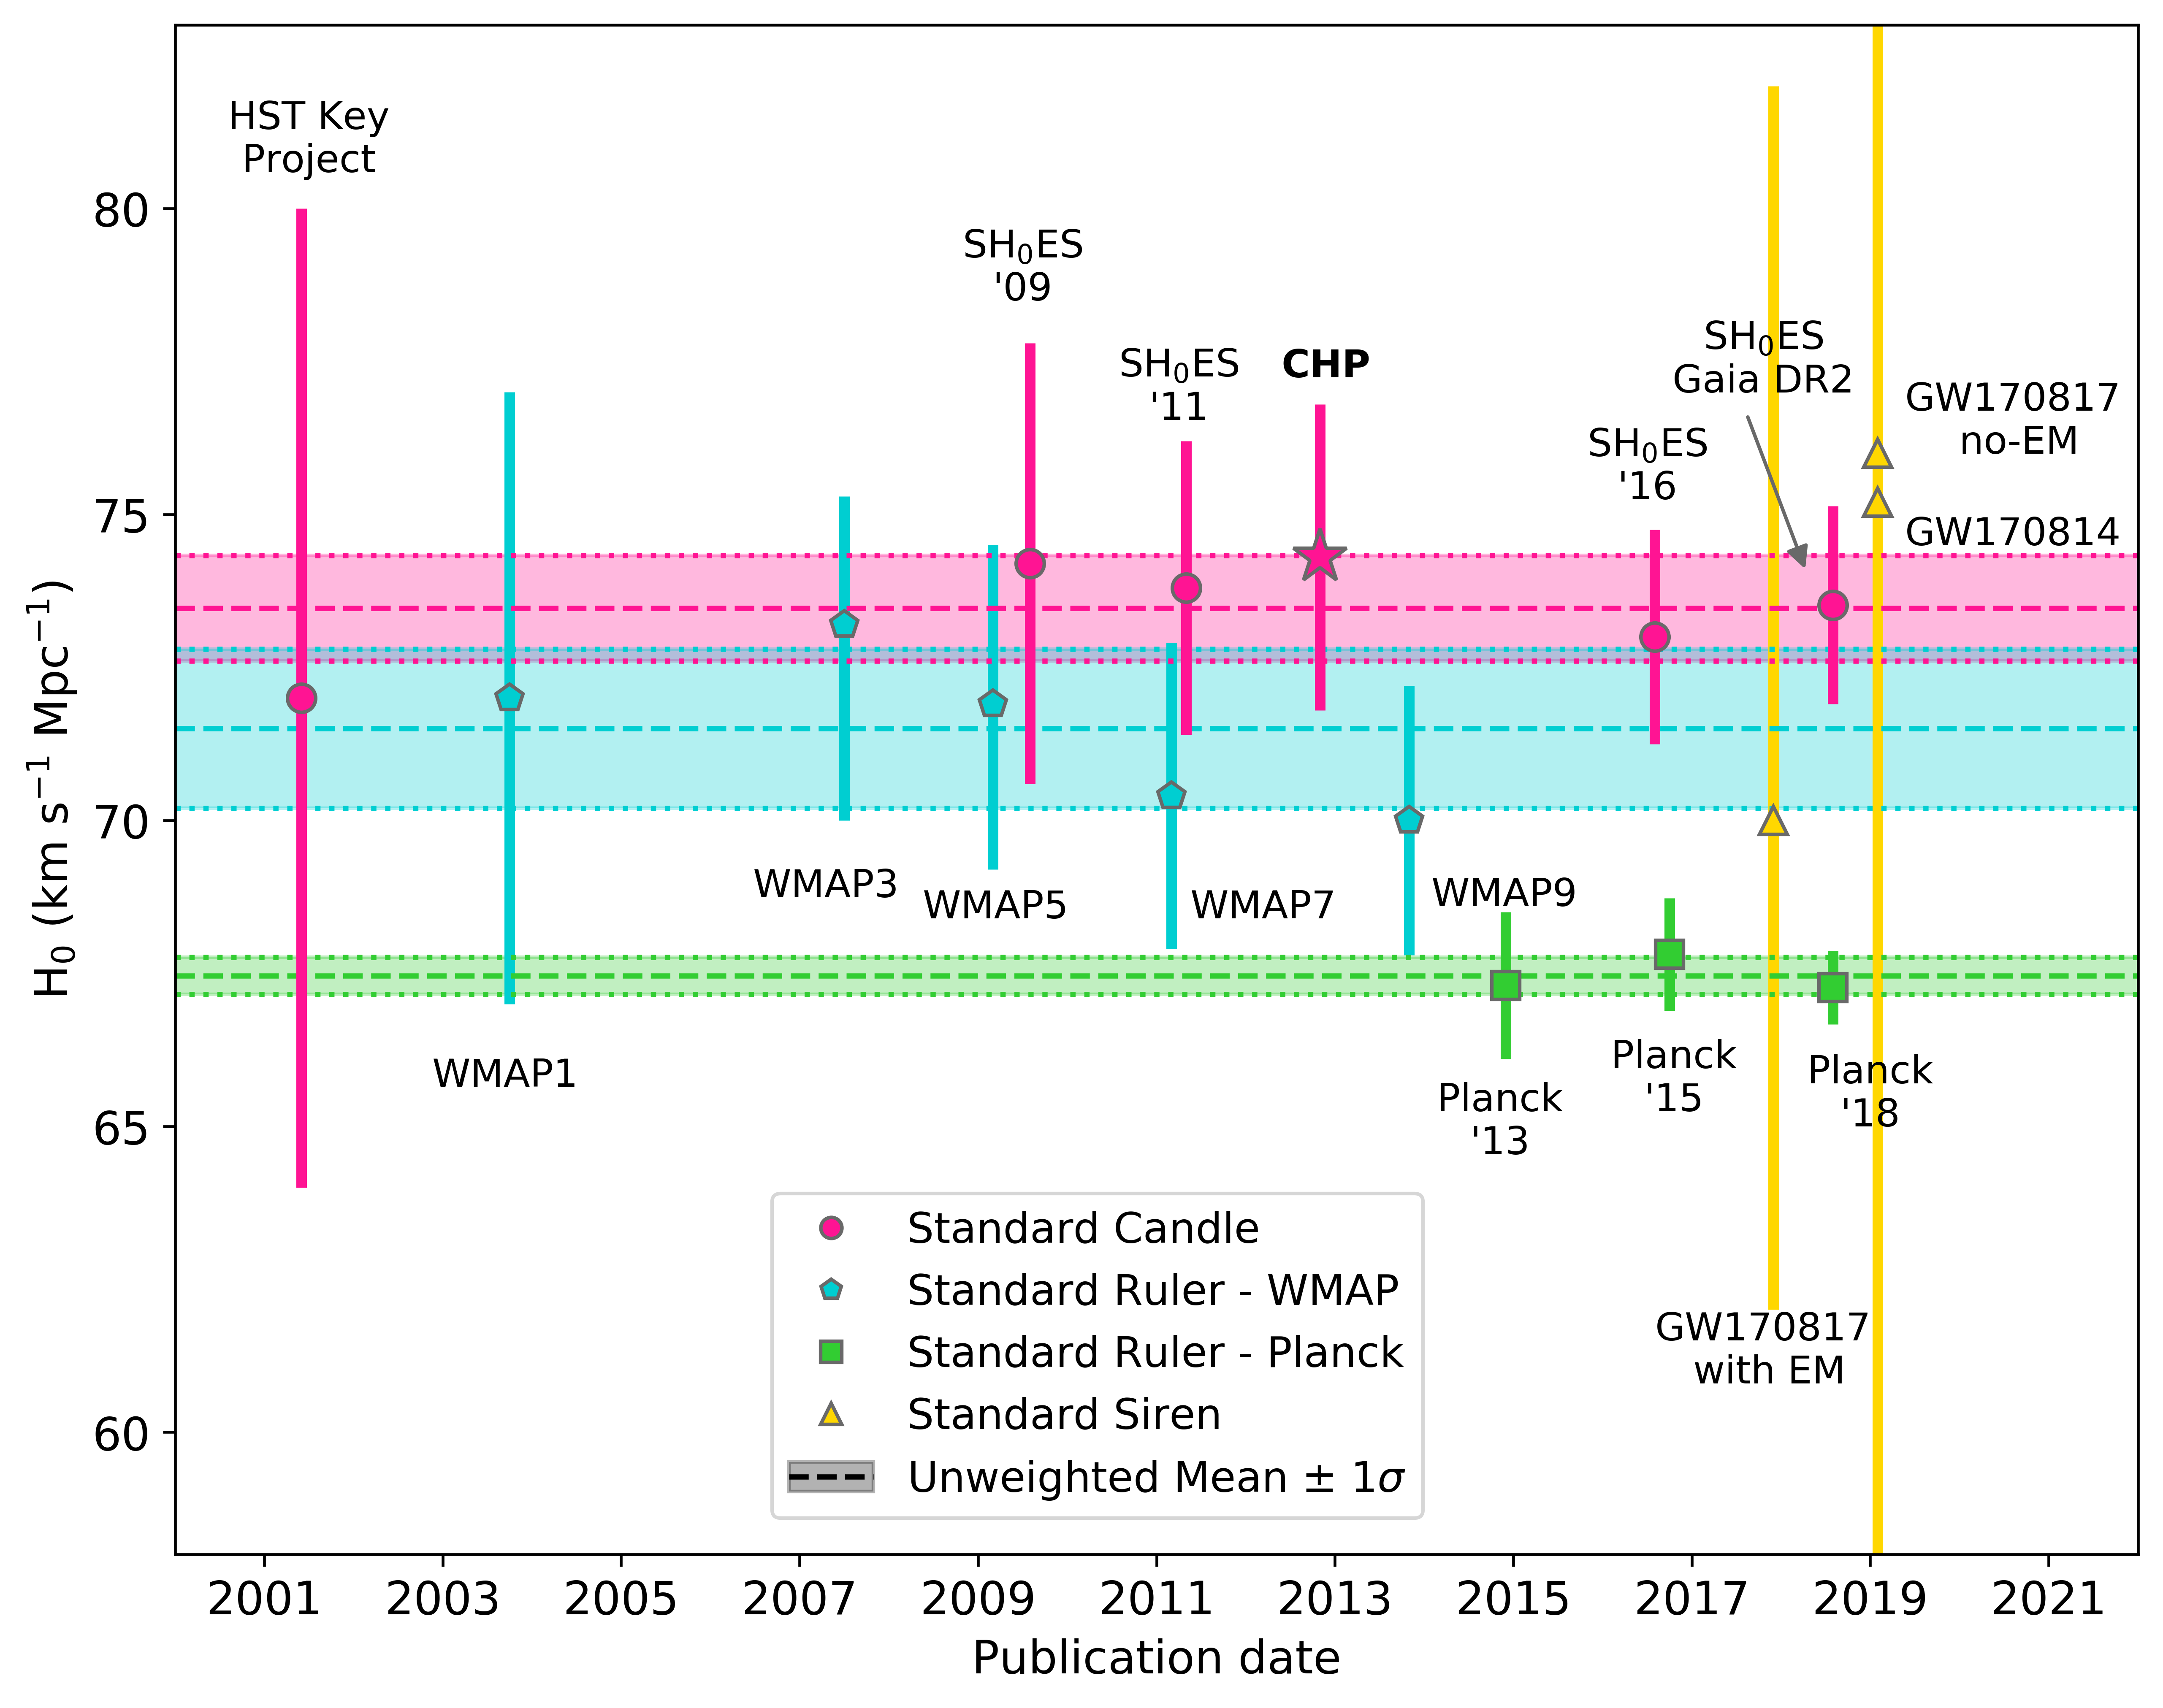
\includegraphics[width=0.7\linewidth]{Images/ho-tension} \caption{This is a figure caption.}\label{fig:ho-plot}
\end{figure}

Important parts of this command:

\begin{itemize}
\tightlist
\item
  \texttt{echo=FALSE} prevents the code being used to display the figure being shown.
\item
  \texttt{ho-plot} is your figure label.
\item
  \texttt{out-width} is the output width of the figure.
\item
  \texttt{fig.cap} is the figure caption.
\item
  \texttt{knitr::include\_graphics} gives the location of the image file.
\end{itemize}

\hypertarget{sec:fig-captions}{%
\section{Figure captions}\label{sec:fig-captions}}

Figure captions are controlled by the \texttt{fig.cap} setting. Your caption should be inside the double quotes. Remember to use \textbackslash{}" to escape any " characters you may use inside your caption.

You can include cross-references and citations inside figure captions. See Sections \ref{sec:fig-nos}, \ref{sec:cross-ref-eqs}, and \ref{sec:tab-syntax} for how to label and cross-reference figures, equations, and tables. Citations are covered in Section \ref{sec:add-cite}.

\hypertarget{sec:fig-nos}{%
\section{Figure numbering and referencing}\label{sec:fig-nos}}

Figures with labels and captions are numbered according to the section (e.g.~Fig \ref{fig:ho-plot} in this case).

To reference a figure use the syntax

\begin{Shaded}
\begin{Highlighting}[]
\NormalTok{\textbackslash{}@ref(fig:label)}
\end{Highlighting}
\end{Shaded}

where \texttt{fig:label} would be \texttt{fig:ho-plot} in this case.

You can cross reference between sections/chapters, so make sure to use unique figure labels.

\hypertarget{sec:equations}{%
\chapter{Equations}\label{sec:equations}}

\hypertarget{sec:add-eqs}{%
\section{Equation syntax}\label{sec:add-eqs}}

The syntax for equations is similar (but not identical) to LaTeX.

LaTeX code:

\begin{Shaded}
\begin{Highlighting}[]
\NormalTok{\textbackslash{}begin\{equation\}}
\NormalTok{\textbackslash{}label\{eqn:friedman\}}
\BaseNTok{    \textbackslash{}left(\textbackslash{}dfrac\{\textbackslash{}dot\{a\}\}\{a\}\textbackslash{}right)^2 + \textbackslash{}dfrac\{kc^2\}\{a^2\} = \textbackslash{}dfrac\{8\textbackslash{}pi G\}\{3\}\textbackslash{}rho }
\NormalTok{\textbackslash{}end\{equation\}}
\end{Highlighting}
\end{Shaded}

Rmd code:

\begin{Shaded}
\begin{Highlighting}[]
\NormalTok{\textbackslash{}begin\{equation\}}
\BaseNTok{    \textbackslash{}left(\textbackslash{}dfrac\{\textbackslash{}dot\{a\}\}\{a\}\textbackslash{}right)^2 + \textbackslash{}dfrac\{kc^2\}\{a^2\} = \textbackslash{}dfrac\{8\textbackslash{}pi G\}\{3\}\textbackslash{}rho}
\NormalTok{(\textbackslash{}#eq:friedman)}
\NormalTok{\textbackslash{}end\{equation\}}
\end{Highlighting}
\end{Shaded}

\begin{equation}
    \left(\dfrac{\dot{a}}{a}\right)^2 + \dfrac{kc^2}{a^2} = \dfrac{8\pi G}{3}\rho
\label{eq:friedman}
\end{equation}

You can also use the latex

\begin{Shaded}
\begin{Highlighting}[]
\NormalTok{\textbackslash{}begin\{align\}}
\NormalTok{...}
\NormalTok{\textbackslash{}end\{align\}}
\end{Highlighting}
\end{Shaded}

format for equations. If you're converting from LaTeX to markdown with pandoc it may convert equations to

\begin{Shaded}
\begin{Highlighting}[]
\NormalTok{\textbackslash{}begin\{aligned\}}
\NormalTok{...}
\NormalTok{\textbackslash{}end\{aligned\}}
\end{Highlighting}
\end{Shaded}

which also works.

\textbf{LaTeX subequations and intertext}

I haven't been able to get subequations and intertext to work in bookdown. LaTeX equations of the form

\begin{Shaded}
\begin{Highlighting}[]
\NormalTok{\textbackslash{}begin\{subequations\}\textbackslash{}begin\{align\}}
\NormalTok{\textbackslash{}vec\{E\} &= \textbackslash{}left( x,t \textbackslash{}right)}
\NormalTok{\textbackslash{}intertext\{and in 3 dimensional space as\}}
\NormalTok{\textbackslash{}vec\{E\} &= \textbackslash{}left( x,y,z,t \textbackslash{}right)}
\NormalTok{\textbackslash{}end\{align\}\textbackslash{}end\{subequations\}}
\end{Highlighting}
\end{Shaded}

should be written as separate equations with the text between written outside the equation environment, e.g.

\begin{Shaded}
\begin{Highlighting}[]
\NormalTok{\textbackslash{}begin\{align\}}
\NormalTok{\textbackslash{}vec\{E\} &= \textbackslash{}left( x,t \textbackslash{}right)}
\NormalTok{\textbackslash{}end\{align\}}
\NormalTok{and in 3 dimensional space as}
\NormalTok{\textbackslash{}begin\{align\}}
\NormalTok{\textbackslash{}vec\{E\} &= \textbackslash{}left( x,y,z,t \textbackslash{}right)}
\NormalTok{\textbackslash{}end\{align\}}
\end{Highlighting}
\end{Shaded}

\hypertarget{sec:eq-nos-labels}{%
\section{Equation numbers and labels}\label{sec:eq-nos-labels}}

The syntax for the maths is the same, but the labelling changes. To label and equation add

\begin{Shaded}
\begin{Highlighting}[]
\NormalTok{(\textbackslash{}#eq:label)}
\end{Highlighting}
\end{Shaded}

just before \texttt{end\{equation\}}. Only equations with labels will be numbered. If you don't want numbers then don't label the equations, but numbers are helpful.

\hypertarget{sec:cross-ref-eqs}{%
\section{Cross referencing equations}\label{sec:cross-ref-eqs}}

The syntax for cross-referencing equations is similar to sections and figures, i.e.

\begin{Shaded}
\begin{Highlighting}[]
\NormalTok{Eqn. \textbackslash{}@ref(eq:friedman) is the Friedman equation}
\end{Highlighting}
\end{Shaded}

will give ``Eqn. \eqref{eq:friedman} is the Friedman equation''.

\hypertarget{sec:maths-captions}{%
\section{Maths in captions}\label{sec:maths-captions}}

R markdown gets a bit finicky about maths/symbols in captions. You may need to use two backslashes to escape symbols in figure captions.

Example of a finicky caption:

\begin{Shaded}
\begin{Highlighting}[]
\BaseNTok{```}
\BaseNTok{\{r echo=FALSE, gaussian, out.width='100%', fig.show='hold', fig.cap="Gaussian uncertainties. }
\BaseNTok{If we measure a value $x$ for a variable that has a true value $\textbackslash{}\textbackslash{}langle x \textbackslash{}\textbackslash{}rangle$ and}
\BaseNTok{uncertainty $\textbackslash{}\textbackslash{}sigma$, there is a 68.3% probability that $x$ will be within }
\BaseNTok{$\textbackslash{}\textbackslash{}langle x \textbackslash{}\textbackslash{}rangle \textbackslash{}\textbackslash{}pm 1\textbackslash{}\textbackslash{}sigma$. There's a 95.4% probability of $x$ being within }
\BaseNTok{$\textbackslash{}\textbackslash{}langle x \textbackslash{}\textbackslash{}rangle \textbackslash{}\textbackslash{}pm 2\textbackslash{}\textbackslash{}sigma$, and 99.7% of $x$ being within  }
\BaseNTok{$\textbackslash{}\textbackslash{}langle x \textbackslash{}\textbackslash{}rangle \textbackslash{}\textbackslash{}pm 3\textbackslash{}\textbackslash{}sigma$."\}}
\BaseNTok{knitr::include_graphics("Images/normal-curve.png")}
\BaseNTok{```}
\end{Highlighting}
\end{Shaded}

\textbackslash{}begin\{figure\}
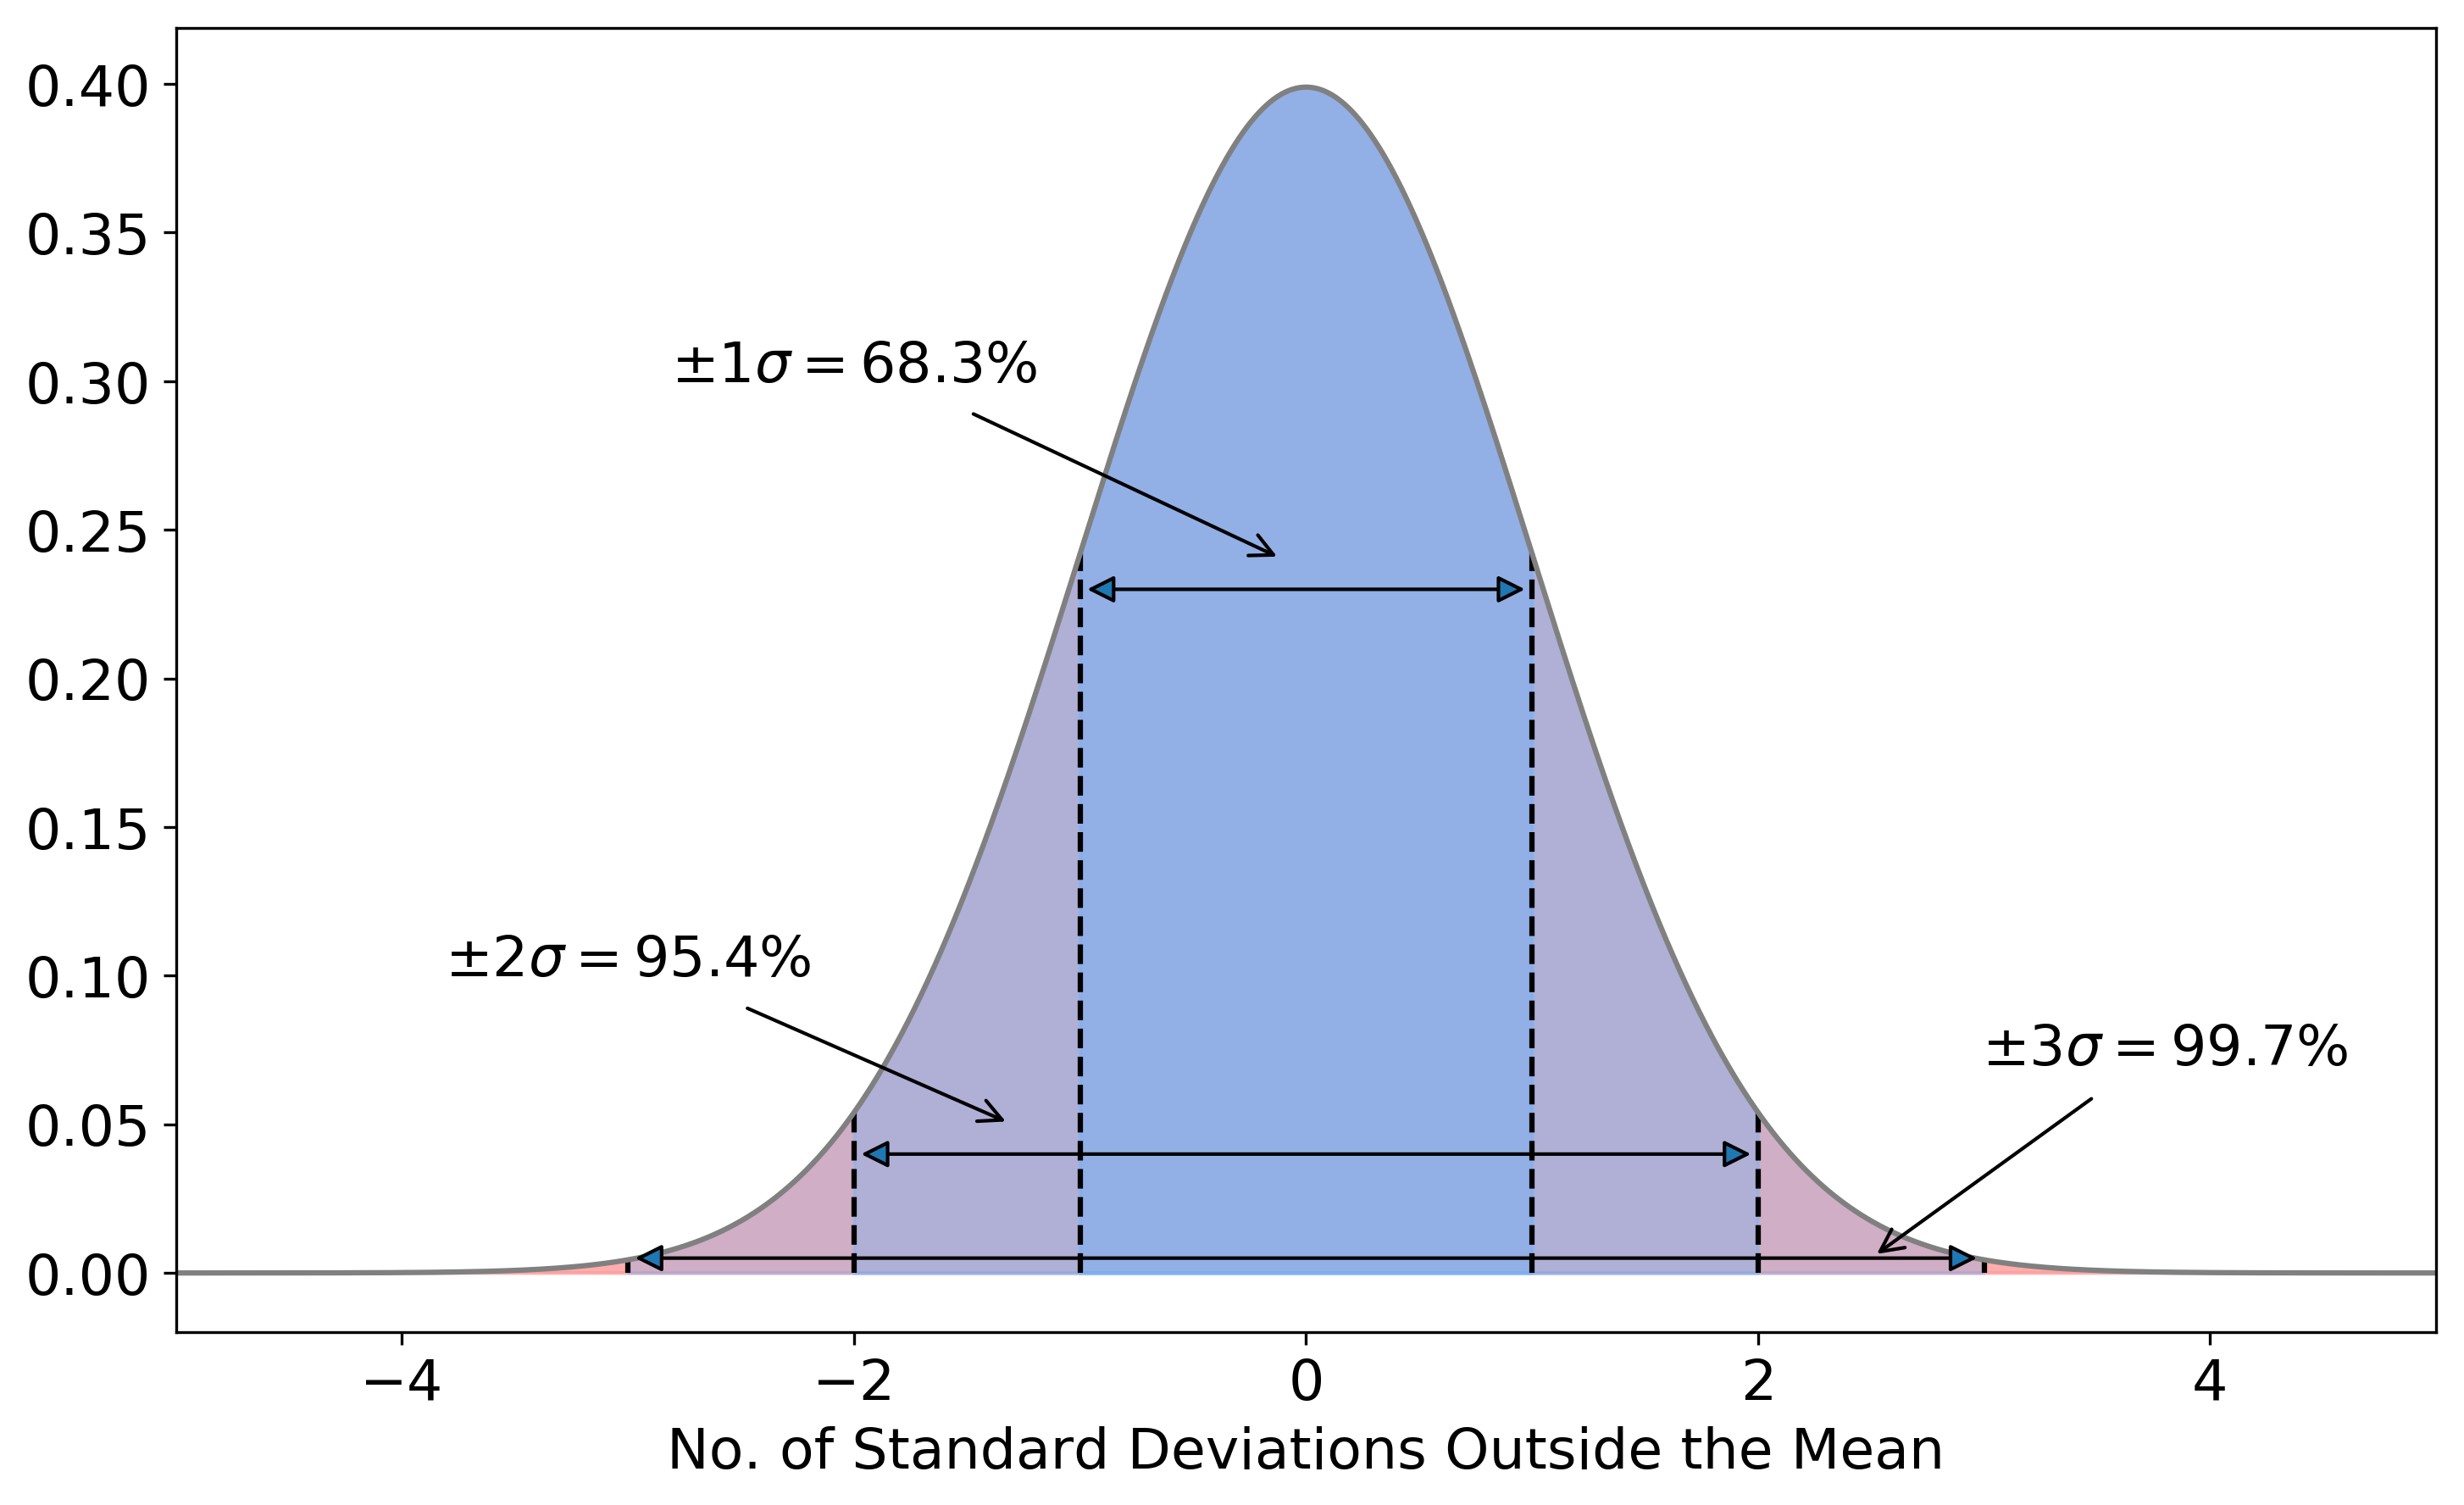
\includegraphics[width=1\linewidth]{Images/normal-curve} \textbackslash{}caption\{Gaussian uncertainties. If we measure a value \(x\) for a variable that has a true value \(\langle x \rangle\) and uncertainty \(\sigma\), there is a 68.3\% probability that \(x\) will be within \(\langle x \rangle \pm 1\sigma\). There's a 95.4\% probability of \(x\) being within \(\langle x \rangle \pm 2\sigma\), and 99.7\% of \(x\) being within \(\langle x \rangle \pm 3\sigma\).\}\label{fig:gaussian}
\textbackslash{}end\{figure\}

\hypertarget{sec:tables}{%
\chapter{Tables}\label{sec:tables}}

\hypertarget{sec:md-tab-gen}{%
\section{Markdown table generator}\label{sec:md-tab-gen}}

If you're making a new table from scratch then the \protect\hyperlink{sec:md-tab-gen}{Markdown Table Generator} (\url{https://www.tablesgenerator.com/markdown_tables}) is a handy tool.

\hypertarget{sec:tab-syntax}{%
\section{Table syntax}\label{sec:tab-syntax}}

Tables are a bit more simple in markdown than in latex. I haven't played around with complex tables much, but it's straightforward to make a basic one.

Example table:

\begin{Shaded}
\begin{Highlighting}[]
\NormalTok{Table: (\textbackslash{}#tab:planck-model) Base $\textbackslash{}Lambda$CDM cosmological parameters from @Planck18. }

\NormalTok{| Parameter | Best fit value     | Uncertainty |}
\NormalTok{|:--------------------|----------:|----------:|}
\NormalTok{| $\textbackslash{}Omega_\{b\}h^2$ | 0.02233 | 0.00015 |}
\NormalTok{| $\textbackslash{}Omega_\{c\}h^2$ | 0.1198 | 0.0012 |}
\NormalTok{| $\textbackslash{}Omega_\{m\}h^2$ | 0.1428 | 0.0011 |}
\NormalTok{| $H_0$ | 67.37 | 0.54 |}
\NormalTok{| $\textbackslash{}Omega_\{m\}$ | 0.3147 | 0.0074 |}
\NormalTok{| Age (Gyr) | 13.801 | 0.024 | }
\NormalTok{| $z_\{re\}$ | 7.64 |  0.74 | }
\NormalTok{| 100$\textbackslash{}theta_\{*\}$ | 1.04108 | 0.00031 | }
\end{Highlighting}
\end{Shaded}

Important things about tables:

\begin{itemize}
\tightlist
\item
  Captions go \textbf{at the top} and should include the label definition.
\item
  Label syntax is \texttt{Table:\ (\textbackslash{}\#tab:table-name)}
\item
  Columns are delimited by \texttt{\textbar{}}
\item
  Justification given by the colons and dashes in the line under the header row.
\end{itemize}

\begin{longtable}[]{@{}lrr@{}}
\caption{\label{tab:planck-model} Base \(\Lambda\)CDM cosmological parameters from \citet{Planck18}.}\tabularnewline
\toprule
Parameter & Best fit value & Uncertainty\tabularnewline
\midrule
\endfirsthead
\toprule
Parameter & Best fit value & Uncertainty\tabularnewline
\midrule
\endhead
\(\Omega_{b}h^2\) & 0.02233 & 0.00015\tabularnewline
\(\Omega_{c}h^2\) & 0.1198 & 0.0012\tabularnewline
\(\Omega_{m}h^2\) & 0.1428 & 0.0011\tabularnewline
\(H_0\) & 67.37 & 0.54\tabularnewline
\(\Omega_{m}\) & 0.3147 & 0.0074\tabularnewline
Age (Gyr) & 13.801 & 0.024\tabularnewline
\(z_{re}\) & 7.64 & 0.74\tabularnewline
100\(\theta_{*}\) & 1.04108 & 0.00031\tabularnewline
\bottomrule
\end{longtable}

\hypertarget{sec:referencing}{%
\chapter{Referencing}\label{sec:referencing}}

\hypertarget{sec:add-cite}{%
\section{Adding citations}\label{sec:add-cite}}

You can reference publications etc using the following syntax:

\begin{Shaded}
\begin{Highlighting}[]
\NormalTok{@bibcode }
\end{Highlighting}
\end{Shaded}

where \texttt{bibcode} is the bibcode for the entry in your bib file (see Sec. \ref{sec:bib-files}). This will give the equivalent of the LaTeX \texttt{\textbackslash{}citet\{\}} command.
Example:

\begin{Shaded}
\begin{Highlighting}[]
\NormalTok{@2016Scowcroft showed that the SMC is a very elongated galaxy.}
\end{Highlighting}
\end{Shaded}

\textbf{\citet{2016Scowcroft} showed that the SMC is a very elongated galaxy.}

For \texttt{\textbackslash{}citep\{\}}, just put the citation in square brackets.

\begin{Shaded}
\begin{Highlighting}[]
\NormalTok{The first observations of SMC Cepheids were taken over 100 years ago [@1912Leavitt].}
\end{Highlighting}
\end{Shaded}

\textbf{The first observations of SMC Cepheids were taken over 100 years ago \citep{1912Leavitt}.}

\hypertarget{sec:bib-files}{%
\section{Bibliography files}\label{sec:bib-files}}

Assuming you're using natbib style references you can pass the same bib file to bookdown.

Example bib file entry:

\begin{Shaded}
\begin{Highlighting}[]
\NormalTok{@ARTICLE\{1912Leavitt,}
\BaseNTok{       author = \{\{Leavitt\}, Henrietta S. and \{Pickering\}, Edward C.\},}
\BaseNTok{        title = "\{Periods of 25 Variable Stars in the Small Magellanic Cloud.\}",}
\BaseNTok{      journal = \{Harvard College Observatory Circular\},}
\BaseNTok{         year = "1912",}
\BaseNTok{       volume = \{173\},}
\BaseNTok{        pages = \{1\},}
\NormalTok{\}}
\end{Highlighting}
\end{Shaded}

\hypertarget{sec:ref-style}{%
\section{Reference style}\label{sec:ref-style}}

The referencing style is controlled in the \texttt{index.Rmd} file.

At the top of this file you'll find the section that defines things like the book title, output format etc. The following lines are where you define the bib file names and referencing format. You can have multiple bib files.

\begin{Shaded}
\begin{Highlighting}[]
\NormalTok{bibliography: [book.bib, packages.bib]}
\NormalTok{csl: apj.csl}
\NormalTok{link-citations: yes}
\end{Highlighting}
\end{Shaded}

The \texttt{bibliography:} line points to your bib file. The \texttt{csl:} line points to your style file. This book uses the ApJ style. Additional style files (e.g.~PRL etc.) can be downloaded from \href{https://www.zotero.org/styles}{zotero}. \texttt{link-citations:\ yes} creates links from the citations in the text to the reference list at the end of the chapter.

Any chapter that includes references will have a the reference list at the end. You can also include a separate reference list for the whole document. To make sure this goes right at the end I usually name my file \texttt{99-references.Rmd}. It should contain the following text:

\begin{Shaded}
\begin{Highlighting}[]

\end{Highlighting}
\end{Shaded}

This will create an \textbf{un-numbered} section at the end of the book called `References' that has the full reference list.

\hypertarget{sec:publishing}{%
\chapter{Publishing}\label{sec:publishing}}

\hypertarget{sec:create-book}{%
\section{Compiling the book}\label{sec:create-book}}

To compile the book, press the `Build Book' button in R Studio. You may need to press the arrow on the button and select \texttt{bookdown::gitbook} the first time you do this.

\begin{figure}

\includegraphics[width=0.5\linewidth]{Images/build-book} \caption{Build book button}\label{fig:build-book}
\end{figure}

This compiles all the markdown to create html files for the book. The output files should be in the \texttt{\_book} folder.

\hypertarget{sec:gh-pages}{%
\section{Publishing with github pages}\label{sec:gh-pages}}

\textbf{THIS SECTION IS NOT COMPLETE}

\textbf{Note:} There is probably a way to do this so that the files are published to somewhere on the University servers. I haven't tried. This is the way I do it.

I use \href{pages.github.com}{github pages} to publish my notes.

The following assumes you are already using github to store your files. \textbf{TODO: Can add instructions for this part if needed}.

Once you have your book on github, create a new branch called \texttt{gh-pages}. This should enable the gh-pages setting in the repo.

Now clone the gh-pages branch into a directory called \texttt{book-output}

\begin{verbatim}
git clone -b gh-pages $repo-path book-output
\end{verbatim}

where \texttt{\$repo-path} is the location of the repository on github, e.g. \texttt{https://github.com/your\_user\_name/lecture\_notes.git/}

Then you want to copy all the output files into this directory and push it to the gh-pages branch.

\begin{verbatim}
cd book-output
cp -r ../_book/* ./
git add --all *
git commit -m "Update the book" || true
git push -q origin gh-pages
\end{verbatim}

Your pretty lecture notes should now be online! You should find them at github\_username.github.io/repo\_name - or check the setting page of the repository. The address will be given in the github pages section.

** TO DO**

Add info on how to update stuff with travis

\bibliography{book.bib,packages.bib}

\end{document}
